\chapter{توازنات الأكسدة والاختزال ومعادلة نرنست}\label{ch:b1:nernst}

ضع صفيحة من الزنك في محلول كبريتات الزنك، وصفيحة من النحاس في
محلول كبريتات النحاس(II)، وصِل المحلولين بأنبوب فيه محلول
ملحي والفلزين بسلك يمر عبر صمام ثنائي باعث للضوء: فيضيء
الصمام. إن تفاعل الزنك مع أيونات النحاس، الذي لا يفعل في
كأس واحدة إلا أن يدفئ المحلول، صار الآن يدفع الإلكترونات في سلك. والبطارية
هي هذا الترتيب نفسه، معبّأً؛ ومقياس pH وقطب
الكلوريد قريباه في القياس. يجعل هذا الفصل تبادل الإلكترونات
قابلًا للحساب: \omterm{def:b1:nernst:oxidation-number}{أعداد الأكسدة} لعدّ الإلكترونات،
\omterm{def:b1:nernst:electrode-potential}{وجهود الأقطاب} لترتيب المزدوجات، \omterm{thm:b1:nernst:nernst}{ومعادلة نرنست}
لتتبعها مع التركيز.

\begin{recall}
عرّف المجلد المدرسي (الصفان الحادي عشر والثاني عشر) المؤكسدات والمختزلات،
وكتب أنصاف المعادلات، وبنى خلايا من فلزين ومحلولين،
وقرأ خلية الزنك--النحاس على أنها بطارية. \omterm{def:b1:extent-q-and-k:quotient}{وخارج التفاعل} وثابت
التوازن هما المعرَّفان في \cref{ch:b1:extent-q-and-k}؛ والنشاطيات
هي $c/c^\circ$ للمذابات و$p/p^\circ$ للغازات، و1 للأجسام الصلبة
والسوائل النقية.
\end{recall}

\section{أعداد الأكسدة والمزدوجات}

\begin{definition}[المؤكسد، المختزل، مزدوجة الأكسدة والاختزال، نصف المعادلة]\label{def:b1:nernst:couple}
\emph{المؤكسد}\index{مؤكسد} نوع كيميائي قادر على اكتساب الإلكترونات،
و\emph{المختزل}\index{مختزل} نوع قادر على منحها. والمؤكسد
Ox والمختزل Red الذي يصير إليه يكوّنان \emph{مزدوجة أكسدة
واختزال}\index{مزدوجة أكسدة واختزال} Ox/Red، توصف
\emph{بنصف معادلتها}\index{نصف معادلة}
$\alpha\,\mathrm{Ox} + n\,\mathrm{e^-} \rightleftharpoons
\beta\,\mathrm{Red}$، الموزونة في الذرات بالماء \ce{H2O} و\ce{H+} عند
الحاجة وفي الشحنة بالإلكترونات.
\end{definition}

تفاعل الأكسدة والاختزال تبادل للإلكترونات بين مزدوجتين:
يُختزل \omterm{def:b1:nernst:couple}{مؤكسد} إحداهما بينما يتأكسد \omterm{def:b1:nernst:couple}{مختزل} الأخرى،
وتُختصر الإلكترونات. ولعدّها في نوع معقد البنية، يُعطى كل
ذرة \omterm{def:b1:nernst:oxidation-number}{عدد أكسدة}.

\begin{definition}[عدد الأكسدة]\label{def:b1:nernst:oxidation-number}
\emph{عدد الأكسدة}\index{عدد الأكسدة} لذرة في
نوع كيميائي هو الشحنة التي كانت ستحملها لو كُسرت كل رابطة معطيةً
إلكتروني الرابطة كليهما للذرة الأكثر كهرسلبية (ويقتسمان بالتساوي
بين ذرتين متماثلتين). ويُكتب بالأرقام الرومانية: الحديد(III)،
و\ce{Mn^{+VII}} في أيون البرمنغنات.
\end{definition}

\begin{proposition}[قواعد أعداد الأكسدة]\label{prop:b1:nernst:on-rules}
\begin{enumerate}
  \item \omterm{def:b1:nernst:oxidation-number}{عدد أكسدة} الذرة في عنصر 0؛ \omterm{def:b1:nernst:oxidation-number}{وعدد أكسدة} الأيون الأحادي الذرة
        شحنته.
  \item مجموع \omterm{def:b1:nernst:oxidation-number}{أعداد أكسدة} ذرات نوع كيميائي يساوي
        شحنته.
  \item الهيدروجين \babelsublr{$+$I} (إلا في هيدريدات الفلزات، حيث \babelsublr{$-$I})؛ والأكسجين
        \babelsublr{$-$II} (إلا في البيروكسيدات، حيث \babelsublr{$-$I}، وحين يرتبط بالفلور)؛ والفلور
        \babelsublr{$-$I}.
  \item في \omterm{def:b1:nernst:couple}{نصف المعادلة} يساوي عدد الإلكترونات تغيرَ
        \omterm{def:b1:nernst:oxidation-number}{عدد أكسدة} العنصر المتغير مضروبًا في
        عدد ذراته.
\end{enumerate}
\end{proposition}

\begin{proof}
1 و2: كسر كل الروابط يحفظ الشحنة، وبين ذرتين متماثلتين
لا يُنقل شيء. 3: الهيدروجين أقل كهرسلبية من كل
لافلز يرتبط به (\cref{ch:b1:periodicity}) وأكثر من الفلزات
القلوية؛ والأكسجين أكثر كهرسلبية من كل العناصر عدا الفلور،
وفي \ce{O-O} يُقسم الزوج المشترك. 4: يحتفظ H وO بعدديهما،
فالذرات الوحيدة التي تتغير شحنتها الوهمية هي ذرات العنصر
المعني، وتظهر الإلكترونات في \omterm{def:b1:nernst:couple}{نصف المعادلة} بالضبط لموازنة
ذلك التغير في الشحنة.
\end{proof}

\begin{method}[أعداد أكسدة نوع كيميائي]\label{met:b1:nernst:oxidation-numbers}
أعطِ H وO وF والأيونات أعدادها المعتادة؛ ويُستنتج عدد الذرة
الباقية من القاعدة 2. ففي \ce{MnO4-}: $x + 4(-2) = -1$، $x = +7$. وفي
\ce{Cr2O7^2-}: $2x - 14 = -2$، $x = +6$. وفي \ce{S4O6^2-} يكون المتوسط
$+2.5$؛ وتُظهر \omterm{def:b1:lewis-resonance-vsepr:lewis}{بنية لويس} نوعين من الكبريت.
\end{method}

\begin{method}[موازنة نصف معادلة]\label{met:b1:nernst:balance-by-on}
\begin{enumerate}
  \item وازن العنصر الذي يتغير عدد أكسدته.
  \item أضف الإلكترونات: تغير \omterm{def:b1:nernst:oxidation-number}{عدد الأكسدة} مضروبًا في
        عدد الذرات.
  \item وازن الشحنة بأيونات \ce{H+} (في محلول حمضي) أو \ce{OH-}
        (في محلول قاعدي).
  \item وازن الهيدروجين والأكسجين بالماء \ce{H2O}؛ وتحقق من الأكسجين أخيرًا.
\end{enumerate}
في أيون البرمنغنات في وسط حمضي: ينتقل Mn من \babelsublr{$+$VII} إلى \babelsublr{$+$II}، فيلزم 5
إلكترونات؛ والشحنة في اليسار $-1 - 5 = -6$ وفي اليمين $+2$،
فيلزم $8\,\ce{H+}$؛ ثم $4\,\ce{H2O}$:
\ce{MnO4- + 8H+ + 5e- -> Mn^2+ + 4H2O}.
\end{method}

\section{الخلايا الكهروكيميائية}

\begin{definition}[الخلية الكهروكيميائية]\label{def:b1:nernst:cell}
\emph{الخلية الكهروكيميائية}\index{خلية كهروكيميائية}
\emph{نصفا خلية}\index{نصف خلية}، يتكوّن كل منهما من مزدوجة
وموصل إلكتروني، هو القطب، يصل بينهما موصل أيوني، كثيرًا ما يكون
\emph{جسرًا ملحيًا}\index{جسر ملحي} (هلامًا أو أنبوبًا فيه ملح خامل مركز
مثل نترات البوتاسيوم). والقطب الذي تجري عنده الأكسدة
هو \emph{المصعد}\index{مصعد}، والذي يجري عنده الاختزال
هو \emph{المهبط}\index{مهبط}. و\emph{جهد
الخلية}\index{جهد الخلية} هو فرق الجهد الكهربائي
بين القطبين، القطب الموجب ناقص القطب السالب، مقيسًا
حين لا يمر أي تيار.
\end{definition}

\begin{omfigure}
\begin{tikzpicture}[font=\small, >={Stealth}]
  \pic at (0,0) {beaker={0.7}{omDef!14}};
  \pic at (3.6,0) {beaker={0.7}{omDef!32}};
  \pic at (-0.3,0.25) {electrode={black!35}};
  \pic at (3.9,0.25) {electrode={orange!70!brown}};
  \pic at (0.35,0.55) {saltbridge={2.9}};
  \pic (m) at (1.8,4.3) {meter={V}};
  \draw[thick] (-0.15,2.65) |- (m-a);
  \draw[thick] (4.05,2.65) |- (m-b);
  \node[anchor=east] at (-0.95,1.0) {\ce{Zn}};
  \node[anchor=west] at (4.45,1.0) {\ce{Cu}};
  \node at (0.25,-0.35) {\ce{Zn^2+}, \ce{SO4^2-}};
  \node at (3.6,-0.35) {\ce{Cu^2+}, \ce{SO4^2-}};
  \draw[->, omProp, thick] (-0.15,3.35) -- (0.8,3.35) node[above, midway] {$\mathrm{e^-}$};
  \draw[->, omProp, thick] (2.8,3.35) -- (3.75,3.35) node[above, midway] {$\mathrm{e^-}$};
  \node[anchor=east] at (-0.9,2.3) {\foreignlanguage{arabic}{$-$ المصعد}};
  \node[anchor=west] at (4.6,2.3) {\foreignlanguage{arabic}{المهبط $+$}};
  \node[font=\scriptsize, align=center] at (1.8,2.75) {الجسر الملحي\\ \ce{K+} $\rightarrow$ \quad $\leftarrow$ \ce{NO3-}};
  \node[font=\scriptsize] at (-0.1,-0.8) {\ce{Zn -> Zn^2+ + 2e-}};
  \node[font=\scriptsize] at (3.7,-0.8) {\ce{Cu^2+ + 2e- -> Cu}};
\end{tikzpicture}

{\small خلية الزنك--النحاس (خلية دانييل). يتأكسد الزنك عند \omterm{def:b1:nernst:cell}{المصعد}،
القطب السالب؛ وتُختزل أيونات النحاس عند \omterm{def:b1:nernst:cell}{المهبط}، القطب
الموجب. وتسري الإلكترونات في الدارة الخارجية من الزنك إلى النحاس؛
وفي \omterm{def:b1:nernst:cell}{الجسر الملحي} تتحرك الكاتيونات نحو \omterm{def:b1:nernst:cell}{المهبط} والأنيونات
نحو \omterm{def:b1:nernst:cell}{المصعد}، فيبقى كل محلول متعادلًا.}
\end{omfigure}

تُكتب الخلية سطرًا، \omterm{def:b1:nernst:cell}{والمصعد} على اليسار: \babelsublr{\ce{Zn} $|$ \ce{Zn^2+}
$\|$ \ce{Cu^2+} $|$ \ce{Cu}}، بخطوط مفردة للحدود الفاصلة وخط مزدوج
\omterm{def:b1:nernst:cell}{للجسر الملحي}. وحين تكون كل التراكيز \qty{1}{mol/L} يكون
جهدها \qty{1.10}{V}. والتفاعل الذي يجري حين تولّد الخلية
تيارًا، \ce{Zn + Cu^2+ -> Zn^2+ + Cu}، هو الذي كان سيحدث في
كأس واحدة؛ وفصل نصفي الخلية يجبر الإلكترونات على المرور في
السلك، حيث يمكنها أن تنجز عملًا.

\section{جهود الأقطاب}

الجهد فرق: فلا يمكن أن تقاس إلا الفروق بين نصفي خلية. ولذلك
يُختار \omterm{def:b1:nernst:cell}{نصف خلية} مرجعي مرة واحدة وإلى الأبد.

\begin{definition}[جهد القطب، الجهد المعياري]\label{def:b1:nernst:electrode-potential}
\emph{قطب الهيدروجين المعياري}\index{قطب الهيدروجين المعياري}
قطب من البلاتين على تماس مع غاز الهيدروجين عند \qty{1}{bar}
ومحلول مثالي لأيونات \ce{H+} نشاطيتها 1. و\emph{جهد
القطب}\index{جهد القطب} $E$ \omterm{def:b1:nernst:cell}{لنصف خلية} هو \omterm{def:b1:nernst:cell}{جهد
الخلية} المكوّنة منه ومن قطب الهيدروجين المعياري على اليسار:
$E = V_{\text{نصف الخلية}} - V_{\text{المرجع}}$. وحين تكون \omterm{def:b1:extent-q-and-k:activity}{نشاطية} كل نوع في
المزدوجة 1، يكون هذا \emph{الجهد المعياري}\index{جهد معياري}
$E^\circ$ للمزدوجة، وهو ثابت عند درجة حرارة معطاة.
\end{definition}

\begin{omfigure}
\begin{tikzpicture}[font=\small, >={Stealth}]
  \pic at (0,0) {beaker={0.72}{omDef!14}};
  % glass jacket, open at the bottom, with the gas inlet on the right
  \draw[om glass] (-0.32,0.35) -- (-0.32,3.0) -- (0.32,3.0) -- (0.32,2.55)
    -- (0.95,2.55) (0.32,2.35) -- (0.95,2.35) (0.32,2.35) -- (0.32,0.35);
  \draw[thick] (0,0.9) -- (0,3.45);
  \fill[black!60] (-0.16,0.5) rectangle (0.16,0.9);
  \foreach \x/\y in {0.45/0.45, 0.55/0.75, 0.48/1.05, -0.45/0.5, -0.52/0.85}
    \draw[omDef!70] (\x,\y) circle (0.055);
  \draw[->] (1.9,2.45) node[right] {\ce{H2}, \qty{1}{bar}} -- (1.0,2.45);
  \draw (0.12,0.7) -- (1.5,0.2) node[right] {بلاتين مبلتن};
  \draw (-0.6,1.1) -- (-1.4,1.6) node[left] {\foreignlanguage{arabic}{\ce{H+}، نشاطية \babelsublr{1}}};
  \node[anchor=west] at (0.05,3.45) {إلى الدارة};
\end{tikzpicture}

{\small \omterm{def:b1:nernst:electrode-potential}{قطب الهيدروجين المعياري}: يتدفق غاز الهيدروجين فقاعاتٍ فوق
صفيحة من البلاتين مكسوّة ببلاتين دقيق، مغموسة في محلول
\omterm{def:b1:extent-q-and-k:activity}{نشاطية} \ce{H+} فيه 1. ومزدوجته $\ce{H+}/\ce{H2}$، وجهدها 0
اصطلاحًا.}
\end{omfigure}

قطب الهيدروجين صعب الاستعمال؛ فتقيس المختبرات بالنسبة إلى
\omterm{def:b1:nernst:cell}{نصف خلية} أيسر استعمالًا جهدُه معلوم.

\begin{definition}[القطب المرجعي]\label{def:b1:nernst:reference-electrode}
\emph{القطب المرجعي}\index{قطب مرجعي} \omterm{def:b1:nernst:cell}{نصف خلية}
جهده ثابت ومعلوم: قطب الفضة--كلوريد الفضة
(سلك من الفضة مكسوّ بكلوريد الفضة في محلول كلوريد ذي
تركيز ثابت) أو قطب الكالوميل (الزئبق على تماس مع
\ce{Hg2Cl2} ومحلول كلوريد).
\end{definition}

يعطي الجدول أدناه \omterm{def:b1:nernst:electrode-potential}{الجهود المعيارية} المستعملة في هذا المجلد؛ ويُظهر
السلّم الرأسي في القسم التالي أكثرها شيوعًا.

\begin{omfigure}
\begin{tabular}{lr@{\qquad}lr}
\hline
المزدوجة & $E^\circ$ (V) & المزدوجة & $E^\circ$ (V) \\
\hline
$\ce{Li+}/\ce{Li}$ & $-3.04$ & $\ce{Cu^2+}/\ce{Cu}$ & 0.34 \\
$\ce{K+}/\ce{K}$ & $-2.94$ & $[\ce{Fe(CN)6}]^{3-}$/$[\ce{Fe(CN)6}]^{4-}$ & 0.36 \\
$\ce{Na+}/\ce{Na}$ & $-2.71$ & $\ce{Cu+}/\ce{Cu}$ & 0.52 \\
$\ce{Mg^2+}/\ce{Mg}$ & $-2.36$ & $\ce{I2}/\ce{I-}$ & 0.53 \\
$\ce{Al^3+}/\ce{Al}$ & $-1.68$ & $\ce{O2}/\ce{H2O2}$ & 0.69 \\
$\ce{Zn^2+}/\ce{Zn}$ & $-0.76$ & $\ce{Fe^3+}/\ce{Fe^2+}$ & 0.77 \\
$\ce{Fe^2+}/\ce{Fe}$ & $-0.41$ & $\ce{Hg2^2+}/\ce{Hg}$ & 0.80 \\
$\ce{Ni^2+}/\ce{Ni}$ & $-0.24$ & $\ce{Ag+}/\ce{Ag}$ & 0.80 \\
$\ce{Pb^2+}/\ce{Pb}$ & $-0.13$ & $\ce{Br2}/\ce{Br-}$ & 1.08 \\
$\ce{H+}/\ce{H2}$ & 0 & $\ce{O2}/\ce{H2O}$ & 1.23 \\
$\ce{S4O6^2-}/\ce{S2O3^2-}$ & 0.02 & $\ce{MnO2}/\ce{Mn^2+}$ & 1.23 \\
$\ce{Cu^2+}/\ce{Cu+}$ & 0.16 & $\ce{Cl2}/\ce{Cl-}$ & 1.36 \\
$\ce{AgCl}/\ce{Ag}$ & 0.22 & $\ce{PbO2}/\ce{Pb^2+}$ & 1.46 \\
$\ce{Hg2Cl2}/\ce{Hg}$ & 0.27 & $\ce{MnO4-}/\ce{Mn^2+}$ & 1.51 \\
 & & $\ce{HClO}/\ce{Cl2}$ & 1.63 \\
 & & $\ce{H2O2}/\ce{H2O}$ & 1.76 \\
\hline
\end{tabular}

\smallskip
{\small \omterm{def:b1:nernst:electrode-potential}{الجهود المعيارية} عند \qty{25}{\celsius}، محسوبة من
طاقات غيبس القياسية المجدولة لتكوين أنواع كل
مزدوجة. وقد تختلف ببضعة أجزاء من مئة من الفولت عن
مجموعات أخرى من القيم.}
% ledger: dfg:Li+_ao, dfg:K+_ao, dfg:Na+_ao, dfg:Mg2+_ao, dfg:Al3+_ao, dfg:Zn2+_ao, dfg:Fe2+_ao, dfg:Ni2+_ao, dfg:Pb2+_ao (computed in figdata/bachelor-1/standard-potentials.py)
% ledger: dfg:S4O62-_ao, dfg:S2O32-_ao, dfg:Cu2+_ao, dfg:Cu+_ao, dfg:AgCl_cr, dfg:Cl-_ao, dfg:Hg2Cl2_cr, dfg:Fe_CN63-_ao, dfg:Fe_CN64-_ao, dfg:I-_ao (same script)
% ledger: dfg:H2O2_ao, dfg:Fe3+_ao, dfg:Hg22+_ao, dfg:Ag+_ao, dfg:Br-_ao, dfg:H2O_l, dfg:MnO2_cr, dfg:Mn2+_ao, dfg:PbO2_cr, dfg:MnO4-_ao, dfg:HClO_ao (same script)
\end{omfigure}

\section{معادلة نرنست}

\begin{theorem}[معادلة نرنست]\label{thm:b1:nernst:nernst}
من أجل مزدوجة $\alpha\,\mathrm{Ox} + n\,\mathrm{e^-} \rightleftharpoons
\beta\,\mathrm{Red}$، مع أنواع أخرى محتملة (\ce{H+}، \ce{H2O}،
\ce{Cl-}) في أي من الطرفين، يُعطى \omterm{def:b1:nernst:electrode-potential}{جهد القطب}
\emph{بمعادلة نرنست}\index{معادلة نرنست}
\[
  E = E^\circ + \frac{RT}{nF}\ln\frac{\prod a_{\text{جهة المؤكسد}}^{\nu}}{\prod
  a_{\text{جهة المختزل}}^{\nu}}
  = E^\circ + \frac{0.059}{n}\log\frac{a(\mathrm{Ox})^\alpha\,\cdots}{a(\mathrm{Red})^\beta\,\cdots}
  \quad\text{عند \qty{25}{\celsius}},
\]
حيث تحمل كل \omterm{def:b1:extent-q-and-k:activity}{نشاطية} عددها الستوكيومتري، والعامل
$RT\ln 10/F = \qty{0.059}{V}$ عند \qty{298}{K}.
\end{theorem}

\admitted{تنتج \omterm{thm:b1:nernst:nernst}{معادلة نرنست} من العلاقة بين طاقة غيبس
للتفاعل \omterm{def:b1:nernst:cell}{وجهد الخلية}، المستخرجة في مجلد السنة
الثانية.}

\begin{example}[ثلاث مزدوجات]\label{ex:b1:nernst:examples}
$\ce{Cu^2+}/\ce{Cu}$: $E = 0.34 + 0.030\log[\ce{Cu^2+}]$ (\omterm{def:b1:extent-q-and-k:activity}{نشاطية} فلز النحاس
1).
$\ce{Fe^3+}/\ce{Fe^2+}$: $E = 0.77 + 0.059\log([\ce{Fe^3+}]/[\ce{Fe^2+}])$.
$\ce{MnO4-}/\ce{Mn^2+}$: $E = 1.51 + \frac{0.059}{5}\log
\frac{[\ce{MnO4-}][\ce{H+}]^8}{[\ce{Mn^2+}]}$؛ وعند تساوي تركيزي
البرمنغنات والمنغنيز(II)، $E = 1.51 - 0.094\,\mathrm{pH}$: فالقدرة
المؤكسدة للبرمنغنات تهبط كلما ارتفع pH.
\end{example}

تغيّر التركيز عشرة أضعاف يزيح الجهد بمقدار $0.059/n$
فولت: بضع عشرات من الميليفولت. ولهذا كان الجهد المقيس بدقة
الميليفولت مقياسًا دقيقًا للتركيز، وهذا مبدأ
قطب pH وقطب الكلوريد في مسألة نهاية الأسبوع.

\begin{history}[فالتر نرنست]
\begin{minipage}[t]{0.22\linewidth}\vspace{0pt}
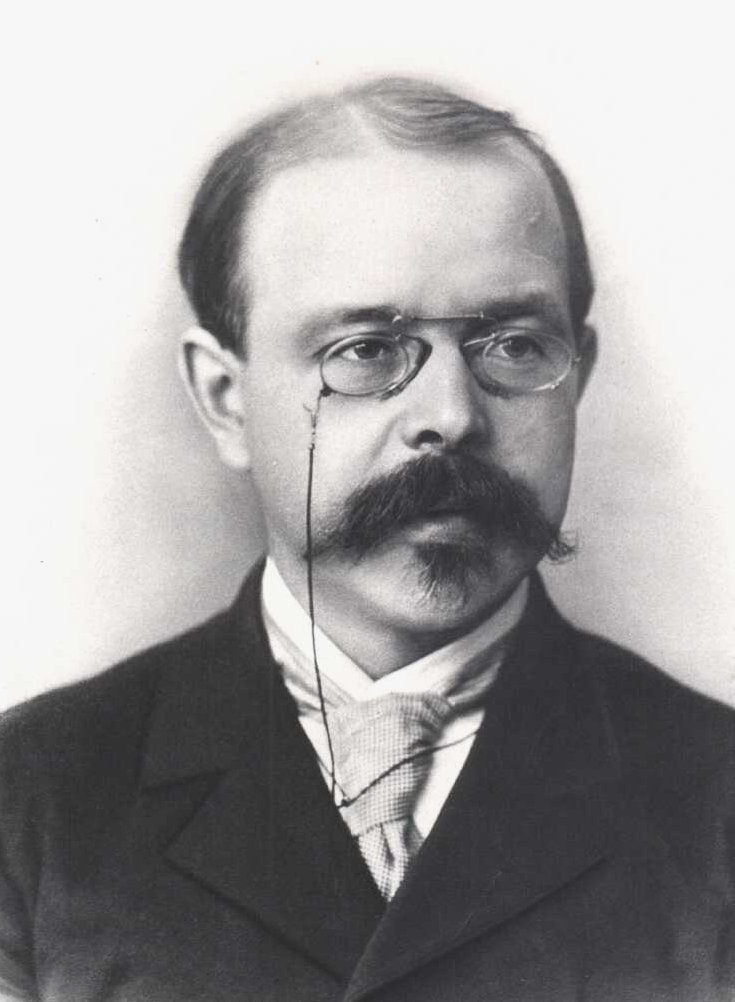
\includegraphics[width=\linewidth]{images/book2/nernst.jpg}
\end{minipage}\hfill
\begin{minipage}[t]{0.74\linewidth}\vspace{0pt}
فالتر نرنست (1864--1941)، هنا في الخامسة والعشرين، سنة 1889. تحمل
معادلة هذا القسم، التي تربط \omterm{def:b1:nernst:cell}{جهد الخلية} بتراكيز
أيوناتها، اسمه، وكذلك المبدأ الثالث
للتحريك الحراري الذي نلقاه في مجلد السنة الثانية. (تصوير: مكتبات
سميثسونيان، ملكية عامة، ويكيميديا كومنز.)
\end{minipage}
\end{history}

\section{التنبؤ بتفاعلات الأكسدة والاختزال}

\begin{method}[التنبؤ بتفاعل أكسدة واختزال]\label{met:b1:nernst:predict-redox}
\begin{enumerate}
  \item ضع المزدوجات على سلّم رأسي \omterm{def:b1:nernst:electrode-potential}{للجهود المعيارية}،
        والمؤكسدات على اليسار، والمختزلات على اليمين.
  \item يتفاعل أقوى \omterm{def:b1:nernst:couple}{مؤكسد} حاضر (أعلى $E^\circ$) مع
        أقوى \omterm{def:b1:nernst:couple}{مختزل} حاضر (أدنى $E^\circ$): فالسهم النازل من
        \omterm{def:b1:nernst:couple}{المؤكسد} إلى \omterm{def:b1:nernst:couple}{المختزل}، ثم الصاعد إلى النواتج، يرسم الحرف
        اليوناني غاما، $\gamma$.
  \item يكون التفاعل مواتيًا ($K > 1$) حين تقع مزدوجة \omterm{def:b1:nernst:couple}{المؤكسد}
        فوق مزدوجة \omterm{def:b1:nernst:couple}{المختزل}؛ ويكون \omterm{def:b1:extent-q-and-k:quantitative}{كمّيًا} عمليًا حين يتجاوز
        الفرق نحو \qty{0.25}{V} لإلكترون واحد متبادَل.
\end{enumerate}
\end{method}

\begin{omfigure}
\begin{tikzpicture}[font=\small, >={Stealth}, y=2.6cm]
  \draw[->, thick] (0,-1.0) -- (0,1.85) node[above] {$E^\circ$ (V)};
  \foreach \e/\o/\r in {-0.76/\ce{Zn^2+}/\ce{Zn}, 0/\ce{H+}/\ce{H2},
      0.34/\ce{Cu^2+}/\ce{Cu}, 0.77/\ce{Fe^3+}/\ce{Fe^2+},
      1.36/\ce{Cl2}/\ce{Cl-}, 1.51/\ce{MnO4-}/\ce{Mn^2+}} {
    \draw (-0.12,\e) -- (0.12,\e);
    \node[anchor=east] at (-0.25,\e) {\o};
    \node[anchor=west] at (0.25,\e) {\r};
    \node[anchor=west, black!55, font=\scriptsize] at (2.0,\e) {\e};
  }
  \node[omProp] at (-1.0,1.85) {المؤكسدات};
  \node[omDef] at (1.1,1.85) {المختزلات};
  % the gamma: Cu2+ meets Zn below it on the other side
  \draw[omThm, very thick, ->, rounded corners=4pt] (-1.0,0.28) -- (-1.0,-0.42) -- (0.6,-0.70);
  \draw[omThm, thick, ->] (-0.5,0.40) to[bend left=40] (0.5,0.40);
  \draw[omThm, thick, ->] (0.5,-0.85) to[bend left=40] (-0.5,-0.85);
\end{tikzpicture}

{\small سلّم \omterm{def:b1:nernst:electrode-potential}{للجهود المعيارية}. قاعدة غاما: يتفاعل \omterm{def:b1:nernst:couple}{المؤكسد}
\ce{Cu^2+} مع \omterm{def:b1:nernst:couple}{المختزل} \ce{Zn} الواقع تحته في الجهة الأخرى
(السهم الغليظ)؛ فيُختزل \ce{Cu^2+} إلى \ce{Cu} (السهم المنحني العلوي)
ويتأكسد \ce{Zn} إلى \ce{Zn^2+} (السهم المنحني السفلي). أما التفاعل العكسي،
\ce{Cu} مع \ce{Zn^2+}، فغير مواتٍ.}
\end{omfigure}

\begin{proposition}[ثابت التوازن انطلاقًا من الجهود المعيارية]\label{prop:b1:nernst:equilibrium-constant}
من أجل التفاعل $\mathrm{Ox_1} + \mathrm{Red_2} \rightleftharpoons
\mathrm{Red_1} + \mathrm{Ox_2}$ الذي يتبادل $n$ إلكترونًا،
\[
  \log K = \frac{n\,(E^\circ_1 - E^\circ_2)}{0.059}\quad\text{عند \qty{25}{\celsius}} .
\]
\end{proposition}

\begin{proof}
عند التوازن لا يمر أي تيار في خلية مبنية من المزدوجتين:
فللقطبين الجهد نفسه، $E_1 = E_2$. لنكتب \omterm{thm:b1:nernst:nernst}{معادلة نرنست}
لكل منهما بالعدد $n$ نفسه: $E^\circ_1 + \frac{0.059}{n}\log
\frac{a(\mathrm{Ox_1})}{a(\mathrm{Red_1})} = E^\circ_2 + \frac{0.059}{n}\log
\frac{a(\mathrm{Ox_2})}{a(\mathrm{Red_2})}$، فيكون $\frac{n(E^\circ_1 -
E^\circ_2)}{0.059} = \log\frac{a(\mathrm{Red_1})a(\mathrm{Ox_2})}{a(\mathrm{Ox_1})
a(\mathrm{Red_2})} = \log K$، والنشاطيات هي نشاطيات التوازن.
\end{proof}

ومن أجل تفاعل دانييل، $\log K = 2(0.34 + 0.76)/0.059 = 37$: فالزنك
يختزل أيونات النحاس اختزالًا تامًا. ومن أجل \ce{2Fe^3+ + 2I- <=> 2Fe^2+ + I2}،
$\log K = 2(0.77 - 0.53)/0.059 = 8.1$. ومنه معيار
الطريقة: مع $n = 1$، يعطي فرق قدره \qty{0.25}{V} القيمة $K = 10^{4.2}$.

\begin{proposition}[تركيب الجهود]\label{prop:b1:nernst:combined-potentials}
إذا تركبت المزدوجتان $\mathrm{A}/\mathrm{B}$ (بعدد $n_1$ من الإلكترونات)
و$\mathrm{B}/\mathrm{C}$ (بعدد $n_2$) في $\mathrm{A}/\mathrm{C}$
($n_3 = n_1 + n_2$)، كان $n_3 E^\circ_3 = n_1 E^\circ_1 + n_2 E^\circ_2$.
فالجهود لا تُجمع؛ أما الجهود المرجَّحة بعدد الإلكترونات فتُجمع.
\end{proposition}

\begin{proof}
في محلول يحوي A وB وC في \omterm{def:b1:extent-q-and-k:quantitative}{حالة توازن} مع قطب واحد،
يكون للمزدوجات الثلاث الجهد نفسه $E$. نضرب \omterm{thm:b1:nernst:nernst}{معادلة نرنست}
للأولى في $n_1$ ومعادلة الثانية في $n_2$ ونجمع: فتُختصر
\omterm{def:b1:extent-q-and-k:activity}{نشاطية} B ويكون $(n_1 + n_2)E = n_1E^\circ_1 + n_2E^\circ_2 +
0.059\log\frac{a(\mathrm{A})}{a(\mathrm{C})}$، وهي $n_3$ مرة
\omterm{thm:b1:nernst:nernst}{معادلة نرنست} للمزدوجة A/C مع $E^\circ_3$ كما ورد.
\end{proof}

النحاس: $2E^\circ(\ce{Cu^2+}/\ce{Cu}) = 0.16 + 0.52 = 0.68$، فيكون
$E^\circ(\ce{Cu^2+}/\ce{Cu}) = 0.34$~V، كما في الجدول. ولأن
$E^\circ(\ce{Cu+}/\ce{Cu}) > E^\circ(\ce{Cu^2+}/\ce{Cu+})$، فإن أيون
النحاس(I) يؤكسد نفسه ويختزلها، \ce{2Cu+ -> Cu^2+ + Cu}: فلا يبقى
في الماء (\cref{ch:b1:e-ph-diagrams}).

\begin{proposition}[قطب من النوع الثاني]\label{prop:b1:nernst:second-kind}
سلك من الفضة مكسوّ بكلوريد الفضة في محلول كلوريد له
الجهد
\[
  E = E^\circ(\ce{AgCl}/\ce{Ag}) - 0.059\log[\ce{Cl-}], \qquad
  E^\circ(\ce{AgCl}/\ce{Ag}) = E^\circ(\ce{Ag+}/\ce{Ag}) - 0.059\,\mathrm{p}K_s(\ce{AgCl}) .
\]
\end{proposition}

\begin{proof}
يكون السلك في \omterm{def:b1:extent-q-and-k:quantitative}{حالة توازن} مع أيونات \ce{Ag+} في المحلول:
$E = E^\circ(\ce{Ag+}/\ce{Ag}) + 0.059\log[\ce{Ag+}]$، ويحدد كلوريد الفضة
$[\ce{Ag+}] = K_s/[\ce{Cl-}]$. وبالتعويض،
$E = E^\circ(\ce{Ag+}/\ce{Ag}) + 0.059\log K_s - 0.059\log[\ce{Cl-}]$.
\end{proof}

وعدديًا $0.80 - 0.059 \times 9.75 = 0.22$~V، وهي قيمة الجدول
المستخرجة على نحو مستقل من طاقات غيبس. ومثل هذا القطب
يقيس الكلوريد، أو يُستعمل، عند تركيز كلوريد ثابت، قطبًا مرجعيًا.

\section{تمارين}

\begin{exercise}[$\star$]\label{exo:b1:nernst:1}
أعطِ \omterm{def:b1:nernst:oxidation-number}{عدد أكسدة} الذرة المسطَّر تحتها: \ce{\underline{N}H3}،
\ce{\underline{N}O3-}، \ce{\underline{S}O4^2-}، \ce{H2\underline{O}2}،
\ce{\underline{Cr}2O7^2-}، \ce{\underline{Cl}O-}، \ce{\underline{Fe}3O4}
(متوسطًا)، \ce{\underline{C}H3OH}.
\end{exercise}

\begin{exercise}[$\star$]\label{exo:b1:nernst:2}
وازن في وسط حمضي أنصاف معادلات $\ce{Cr2O7^2-}/\ce{Cr^3+}$،
$\ce{H2O2}/\ce{H2O}$، $\ce{O2}/\ce{H2O2}$ و$\ce{SO4^2-}/\ce{SO2}$.
\end{exercise}

\begin{exercise}[$\star$]\label{exo:b1:nernst:3}
اكتب \omterm{thm:b1:nernst:nernst}{معادلة نرنست} للمزدوجات $\ce{Zn^2+}/\ce{Zn}$ و$\ce{Cl2}/\ce{Cl-}$
و$\ce{O2}/\ce{H2O}$ و$\ce{Hg2Cl2}/\ce{Hg}$. واحسب جهد صفيحة من الزنك
في كبريتات الزنك تركيزها \qty{0.010}{mol/L}.
\end{exercise}

\begin{exercise}[$\star$]\label{exo:b1:nernst:4}
تحوي خلية دانييل \ce{Zn^2+} بتركيز \qty{0.10}{mol/L} و\ce{Cu^2+} بتركيز
\qty{0.010}{mol/L}. احسب جهد كل قطب، \omterm{def:b1:nernst:cell}{وجهد
الخلية}، وبيّن أي القطبين هو \omterm{def:b1:nernst:cell}{المصعد}.
\end{exercise}

\begin{exercise}[$\star\star$]\label{exo:b1:nernst:5}
وازن \ce{MnO4- + Fe^2+} في وسط حمضي، واحسب ثابت توازنه
وبيّن هل يمكن أن يُستعمل في معايرة.
\end{exercise}

\begin{exercise}[$\star\star$]\label{exo:b1:nernst:6}
أي هذه الفلزات يذوب في حمض تركيزه \qty{1}{mol/L} ليس هو
نفسه مؤكسدًا (حمض الكلوريدريك)، معطيًا الهيدروجين: Mg، Zn، Fe، Ni،
Pb، Cu، Ag؟ اكتب التفاعلات واحسب $\log K$ للمغنيسيوم
وللحديد.
\end{exercise}

\begin{exercise}[$\star\star$]\label{exo:b1:nernst:7}
تستعمل معايرات اليود التفاعل \ce{I2 + 2S2O3^2- -> 2I- + S4O6^2-}. احسب
ثابته من الجدول. هل هو كمّي؟
\end{exercise}

\begin{exercise}[$\star\star$]\label{exo:b1:nernst:8}
انطلاقًا من $E^\circ(\ce{Fe^2+}/\ce{Fe}) = -0.41$~V و$E^\circ(\ce{Fe^3+}/\ce{Fe^2+})
= 0.77$~V، احسب $E^\circ(\ce{Fe^3+}/\ce{Fe})$. وبيّن أن أيونات الحديد(III)
تتفاعل مع فلز الحديد واحسب الثابت.
\end{exercise}

\begin{exercise}[$\star\star$]\label{exo:b1:nernst:9}
بيّن أن جهد المزدوجة $\ce{O2}/\ce{H2O}$ تحت \qty{1}{bar}
من الأكسجين هو $1.23 - 0.059\,\mathrm{pH}$، وأن جهد $\ce{H+}/\ce{H2}$
تحت \qty{1}{bar} من الهيدروجين هو $-0.059\,\mathrm{pH}$. ما
\omterm{def:b1:nernst:cell}{جهد خلية} وقود هيدروجين--أكسجين؟ وهل يتعلق بقيمة pH؟
\end{exercise}

\begin{exercise}[$\star\star\star$]\label{exo:b1:nernst:10}
أيون النحاس(I). بيّن مستعينًا بالجدول أن \ce{Cu+} يخضع لعدم التناسب
في الماء، واحسب ثابت \ce{2Cu+ <=> Cu^2+ + Cu}،
وتركيز \ce{Cu+} الباقي في \omterm{def:b1:extent-q-and-k:quantitative}{حالة توازن} مع فلز النحاس
و\ce{Cu^2+} بتركيز \qty{0.10}{mol/L}.
\end{exercise}

\begin{exercise}[$\star\star\star$]\label{exo:b1:nernst:11}
للخلية \babelsublr{\ce{Ag} $|$ \ce{Ag+} (\qty{1.0e-3}{mol/L}) $\|$ \ce{Ag+}
(\qty{0.10}{mol/L}) $|$ \ce{Ag}} المزدوجة نفسها في الجهتين.
احسب جهدها، وعيّن قطبيها، وصف كيف تتطور
التراكيز وهي تولّد التيار. ومتى تتوقف؟
\end{exercise}

\begin{exercise}[$\star\star\star$]\label{exo:b1:nernst:12}
بيروكسيد الهيدروجين. احسب من الجدول ثابت
\ce{2H2O2 -> 2H2O + O2}، وفسّر لماذا تبقى قارورة بيروكسيد الهيدروجين
مع ذلك مستقرة أشهرًا. أي مزدوجة في الجدول تجعله
مؤكسدًا، وأيها تجعله مختزلًا؟
\end{exercise}

\section{مسألة: القطب الذي يقيس الكلوريد}

\begin{problem}[{مسألة نهاية الأسبوع --- أعداد الأكسدة في مزدوجة
كلوريد الفضة، وخلية مقابل قطب الهيدروجين، وقياس
الكلوريد في عيّنة ماء، والجهد المعياري لقطب
الفضة--كلوريد الفضة}]
\label{pb:b1:nernst:1}
يقيس مختبر للمياه الكلوريد بسلك من الفضة مكسوّ بكلوريد
الفضة، مغموس في العيّنة وموصول \omterm{def:b1:nernst:reference-electrode}{بقطب مرجعي}.
معطيات عند \qty{25}{\celsius}: $E^\circ(\ce{Ag+}/\ce{Ag}) = 0.80$~V،
$E^\circ(\ce{AgCl}/\ce{Ag}) = 0.22$~V، $E^\circ(\ce{Hg2Cl2}/\ce{Hg}) =
0.27$~V، $\mathrm{p}K_s(\ce{AgCl}) = 9.75$، $RT\ln 10/F = 0.059$~V،
$M(\ce{Cl}) = \qty{35.5}{g/mol}$.

\medskip
\noindent\textbf{الجزء الأول --- المزدوجة.}
\begin{enumerate}
  \item أعطِ \omterm{def:b1:nernst:oxidation-number}{عدد أكسدة} الفضة في Ag و\ce{Ag+} و\ce{AgCl}،
        \omterm{def:b1:nernst:oxidation-number}{وعدد أكسدة} الكلور في \ce{AgCl} و\ce{Cl-}.
  \item اكتب \omterm{def:b1:nernst:couple}{نصف معادلة} المزدوجة $\ce{AgCl}/\ce{Ag}$.
  \item اكتب \omterm{thm:b1:nernst:nernst}{معادلة نرنست} الخاصة بها.
  \item فسّر لماذا لا يتعلق الجهد إلا بتركيز
        الكلوريد.
  \item ما \omterm{def:b1:nernst:electrode-potential}{جهد القطب} في كلوريد تركيزه \qty{1.0}{mol/L}؟
  \item احسبه في كلوريد تركيزه \qty{0.010}{mol/L}.
\end{enumerate}

\medskip
\noindent\textbf{الجزء الثاني --- خلية مقابل قطب الهيدروجين.}
\begin{enumerate}[resume]
  \item اكتب الخلية المكوّنة من \omterm{def:b1:nernst:electrode-potential}{قطب الهيدروجين المعياري}
        وقطب كلوريد الفضة في كلوريد تركيزه \qty{0.10}{mol/L}.
  \item أي القطبين هو القطب الموجب؟
  \item احسب \omterm{def:b1:nernst:cell}{جهد الخلية}.
  \item اكتب التفاعل الذي يجري حين تولّد الخلية التيار.
  \item احسب ثابت توازنه.
  \item في أي اتجاه تتحرك الإلكترونات في السلك؟
\end{enumerate}

\medskip
\noindent\textbf{الجزء الثالث --- قياس الكلوريد.}
المرجع قطب كالوميل في كلوريد البوتاسيوم تركيزه \qty{1.0}{mol/L}.
\begin{enumerate}[resume]
  \item ما جهد \omterm{def:b1:nernst:reference-electrode}{القطب المرجعي}؟
  \item من أجل عيّنة كلوريدها \qty{1.0e-3}{mol/L}، أي القطبين هو
        القطب الموجب، وما الجهد؟
  \item عبّر عن الجهد $U$ (قطب الفضة ناقص المرجع) دالةً
        في $[\ce{Cl-}]$.
  \item تعطي عيّنة $U = \qty{0.115}{V}$. احسب تركيز الكلوريد فيها
        بالوحدة \unit{mol/L} وبالوحدة \unit{mg/L}.
  \item أي خطأ نسبي في التركيز يعطيه خطأ قدره \qty{1}{mV} في $U$؟
  \item دون أي تركيز للكلوريد يكف القطب عن
        اتباع \omterm{thm:b1:nernst:nernst}{معادلة نرنست}، إذ يذوب كلوريد الفضة الذي عليه؟
\end{enumerate}

\medskip
\noindent\textbf{الجزء الرابع --- من أين تأتي القيمة 0.22 V؟}
\begin{enumerate}[resume]
  \item اكتب \omterm{thm:b1:nernst:nernst}{معادلة نرنست} للمزدوجة $\ce{Ag+}/\ce{Ag}$.
  \item في وجود كلوريد الفضة الصلب، عبّر عن $[\ce{Ag+}]$ دالةً
        في $[\ce{Cl-}]$.
  \item استنتج جهد سلك الفضة دالةً في
        $[\ce{Cl-}]$.
  \item عيّن $E^\circ(\ce{AgCl}/\ce{Ag})$ في هذه العبارة.
  \item احسبه انطلاقًا من $E^\circ(\ce{Ag+}/\ce{Ag})$ و$\mathrm{p}K_s$،
        وقارنه بقيمة الجدول.
  \item اذكر \omterm{def:b1:nernst:electrode-potential}{الجهد المعياري} لقطب الفضة--كلوريد الفضة
        بمنزلتين عشريتين.
\end{enumerate}
\end{problem}
